\documentclass{business-covered} % A4 paper and 11pt font size


\usepackage{tikz}
\usetikzlibrary{shapes,arrows, positioning}
\usepackage{cite}
\usepackage{hyperref}

\name{GLR}
\maintitle{Hipparcos Catalog}
\generalpurpose{Completeness}
\subtitle{An Analysis of the completeness of the Hipparchus Catalog}
\business{University of Turku}
\recipient{}
\authored{Kristen Elise Gardner}
\department{Department of Physics}
\exhibit{000}
\filing{}
\location{Turku, Finland}
\DOC{15 December 2022}





\begin{document}	
	\section{Motivation}
		The Hipparcos catalog - containing about 118 thousand stars - was created using the European Space Agency's Hipparcos satellite in the early 1990's (Hipparcos being an acronym for "\textbf{Hi}gh \textbf{P}recision \textbf{Par}allax \textbf{Co}llecting \textbf{S}atellite"). Being of historical interest - the acronym is in honor of the greek astronomer Hipparchus, who cataloged some 850 stars in his life - it is pertinent to ask how the Hipparcos catalog fairs in terms of its descriptiveness of our neighborhood of the galaxy. While the catalog has become something of a relic due to advancements in telescope/satellite technology, as well as followup missions meant to map more of the celestial sphere, the purpose of this report will be to analyze the catalog and conclude as to whether or not it is sufficient over some region of neighboring space to be called  accurate and complete across that region. Within the same realm, we will see whether or not our analysis dredges up any interesting information that will either be revelatory to the nature of our neighborhood of the galaxy, or otherwise to the operation/bias of the satellite itself, or to the astronomers that dictated what objects the satellite would study.
		\subsection{Summary of Purpose}
		In summary, the mission of this exploration is two-fold:
		
		\begin{enumerate}
			\item Find the region of space, if any exists, over which the Hipparcos catalog appears to be complete.
			\item Expound upon any interesting discoveries along the way.
		\end{enumerate}

\pagebreak
	\section{Preliminary Study}
		This section will contain some background/technical information concerning the mission, the satellite, and the catalog - in that order - in order to form a more complete sense of the purpose for the reader. This section can be skipped for those whose interest is focused more on the results of the study as a whole, but we include it none-the-less.
		\subsection{The Hipparcos Mission}
			
			The Hipparcos mission - named after the Greek astronomer Hipparchus -  was originally imagined by CNES - the French space agency - to solve the increasingly insurmountable barrier to the improvement of measurements taken from the surface of the earth - atmosphere, gravitational flexing of instruments, etc. The earliest known reference to the idea in the mainstream is the submission of a formal proposal to CNES in 1967. Given the complexity of such a system - necessary in order to achieve a reasonable chance of success - CNES moved the proposal onto the international stage. The mission was eventually accepted by the European Space Agency with the goal of providing galactic positions, parallaxes, and proper motions of nearly 120 thousand stars with a target accuracy of 2 milli-arcseconds (a goal that was inevitably surpassed).
	
\pagebreak
		\subsection{The Hipparcos Satellite}
			The Hipparcos satellite itself was devised in the early 1980 with the mission stated above. It was outfitted with a 29cm aperture Schmidt telescope. Its optical system, the complexity of which was the motivation for the original escalation of the project to a multinational affair, was comprised of two mirrors which created a sort of stereoscopic vision that allowed for absolute parallax measurement - as opposed to the relative measurements generally discussed where in two measurements are taken from the earth from two known locations relative to the sun. This setup ended up allowing the satellite to achieve a median accuracy of around 0.001 arcseconds.
			\begin{figure}[h!]
				\centering
				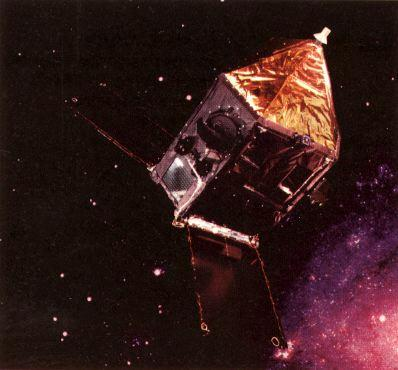
\includegraphics[scale=1]{figures/hipparchos.jpg}
				\caption{The Hipparcos Satellite \cite{nasa}}
			\end{figure}
			The satellite itself had a launch mass of 1,140 kg (naturally with a much lower payload mass of only 210 kg), and was equipped with hydrazine maneuvering thrusters, cold gas attitude thrusters, and a gyroscopic attitude bearing system. The satellite was launched on the 8th of August in 1989, and was deactivated 4 years later after completing its mission on the 15th of August, 1993.
		
\pagebreak
		\subsection{The Hipparcos Catalog}
			
			The Hipparcos Catalog was produced 4 years after the decommissioning of the satellite (published 1997), and boasted a high-precision population of 118,200 stars. While the Tycho Catalog was published simultaneously, it hosted a lower-precision population - though to it's credit it did host a major larger population of 2.5 million stars.
			
			The mission used a pre-formed list of stars called the "Hipparcos Input Catalog", which was simply a list of stars that astronomers planned to observe using the satellite. From this list, 58,00 objects that met one of the following conditions were studied as completely as possible:
				\begin{itemize}
					\item For ST earlier than G5: $M_V < 7.9 +1.1\sin|b|$
					\item For ST later than G5: $M_V < 7.3 +1.1\sin|b|$
				\end{itemize}
		where $b$ is the Galactic latitude. We can extrapolate an upper and lower bound of $6.2 < M_V < 8.4$; while this doesn't necessarily capture every star (there may be a selection of examples which have a spectral type earlier than G5 with a magnitude as high as 9 that would still be included.
		
		The data comprising the catalog was the result of an analysis performed by two independent European teams (NDAC and FAST), which pertained of more than 120 GB of data acquired over the 3.5 year life of the satellite's mission.
		
		For the purpose of this project, we obtained the complete Hipparcos catalog from Vizier. \cite{vizier} Most of the data used in this analysis is direct from the Vizier database, but the distances provided there are all in parallax and, due to the nature of this analysis, we used these values to calculate the distances in parsecs (pc), which is strictly what will be used through this report.		
		
\pagebreak
	\section{Introduction}
		\subsection{Approximate Completeness}
		The easiest way to analyze how complete a star catalog is within some region of space is to look at the distribution of stars it presents within that region, and compare it to the distribution we would expect to find. Now, we may not know what the exact distribution of stars within that region of space is, but we can base a conclusion on some set of basic assumptions regarding the \textit{nature} of that distribution:
			\begin{enumerate}
				\item Stars are uniformly distributed within small regions of galactic 							space.
				\item It is unlikely that the distribution of stars within the Hipparcos catalog will be uniform within some region of space unless it is a complete catalog of that region. (The case of the distribution not being uniform )
			\end{enumerate}
	\subsection{Procedures}
		We will not be measuring the \textit{absolute} completeness of the Hipparcos, as that is, at this point, probably already known, and is generally outside of the scope of this project in so far as more external information would be needed then is necessary to complete this exercise. Thus, we will instead be attempting to measure whether or not the Hipparcos catalog \textbf{can} be complete, by comparing the distribution of stars to the assumption that that distribution should be linear. In the case where the catalog is incomplete, as we expect atleast at some certain distance, we should be able to approximate how many stars are missing from the catalog within that range.
		
		To do this, we will first take the subset of the Hipparcos catalog where $D<=400 pc$, where we calculate the distance $D$ from the given parallax value for each star. We can change this limit if we find that the distribution is fairly uniform when we perform our analysis, this bound is simply a starting point. 
		With this subset, we will create a histogram of the distances, which will give us a rough idea of how the stars are distributed. With this, if we are expecting to see a relatively constant density of stars through our region bounded by 400 pc, then we should see a triangular distribution (i.e. a histogram bounded by a line $N=2\pi mr$, where $m$ is a sort of linear density. I like to think of this linear density as though we were to take some region of space and draw a ray of length $d$ through it: some consistent number of stars will fall on that line, and that number will be proportional to $m$. To the same extent, if we draw a circle of some radius $r$, then we expect to have some number of stars that lie on the circumference of said circle, hence we get the total count of stars at some distance $r$ from Sol to be $N=2\pi mr$.
		The slope of this line doesn't much matter to us outside of the contexts of the straight line suggesting that there is a decent level of completion to the catalog, and in the approximation of the density of stars within our local neighborhood.  		
		Something we need to consider are the error values on the distance measurements - which I believe will be the trickiest part of this analysis. Suppose we obtain a distribution of stars which reveals a non-constant density - which would be represented by a histogram distribution that did not resemble a triangle. We may find that the errors on the parallax would allow for stars to "fall in line", as it were, to allow for the distribution that matches our assumption. Even in the case where the distances calculated directly from the parallax values were to give rise immediately to an apparent uniformity to the distribution, we would still have to consider a confidence based on these errors. Therefore, we will also have to analyze the standard errors on the parallax in order to establish the level of confidence. While calculating a confidence level lies outside of the scope of this exercise - such a task deserves a solid year of further considerations of the data in order to erect a good result - we will use this graphical analysis to gain atleast an idea of our degree of belief in whether the catalog is complete or not.
		
\pagebreak
	\section{Results}
	
		First, let us look at the distribution of distances:
		\begin{figure}[h!]
			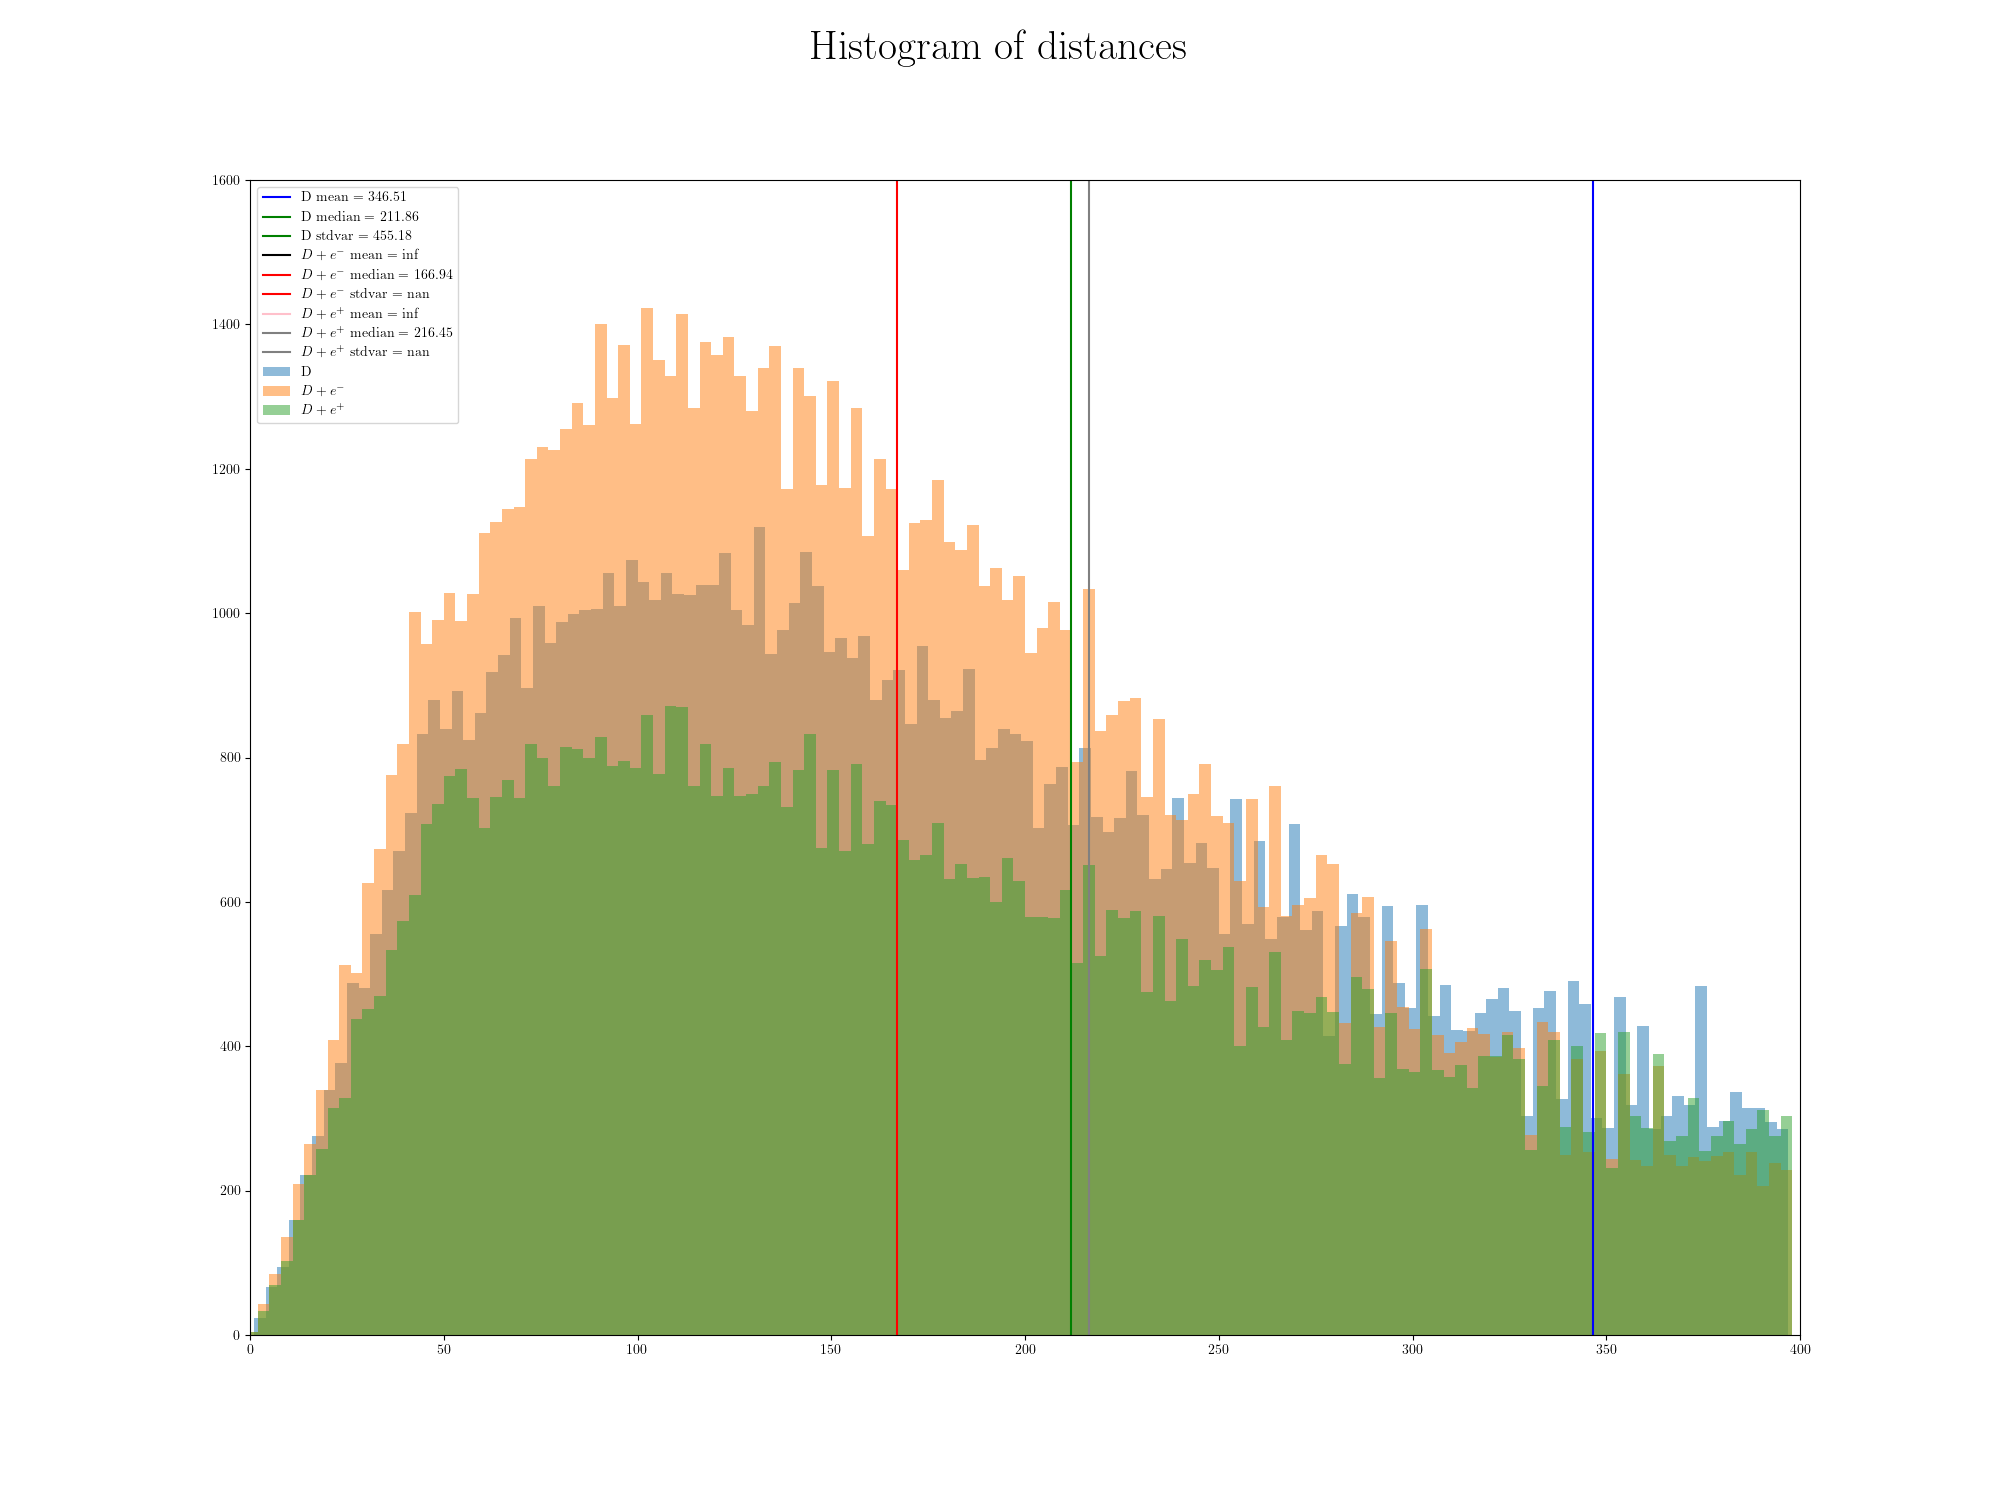
\includegraphics[scale=.33]{figures/dist_hist_base.png}
			\caption{Distance Histogram}
		\end{figure}
		
		From our primitive error comparison-based analysis, we can see that there is a decent possibility that their exists completeness of the catalog upto about 60 pc in general. However, we are looking at the entire set of stars. If we group the stars together by absolute magnitude, we get the following:
		\pagebreak 
		\begin{figure}[h!]
			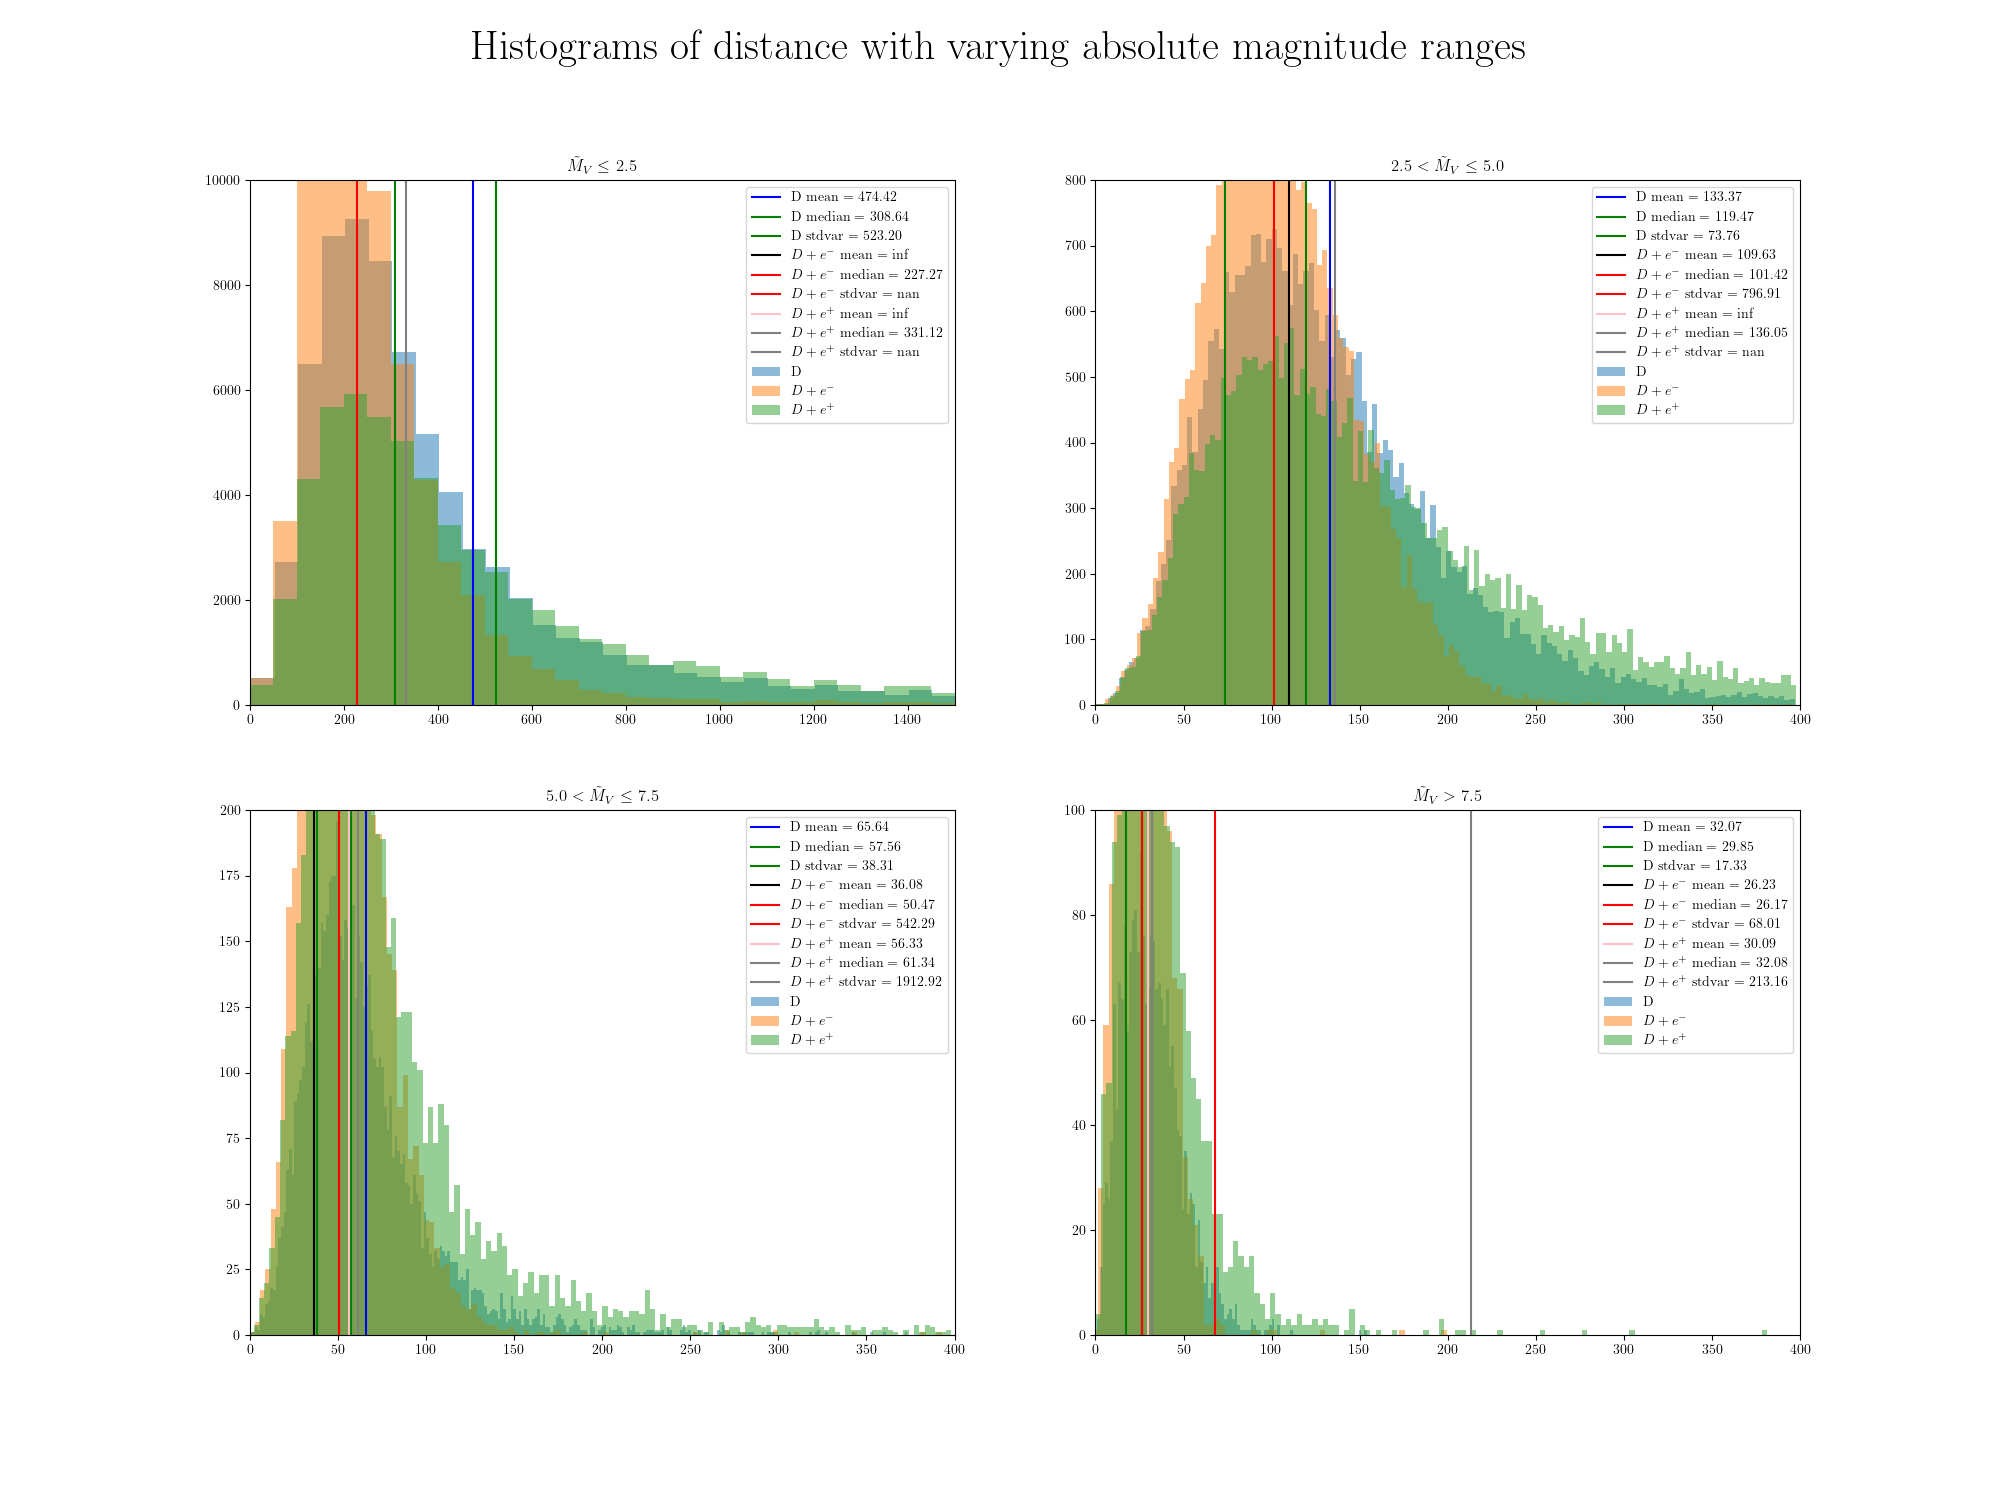
\includegraphics[scale=.33]{figures/dist_hist.png}
			\caption{Distance Histogram (with magnitudinal ranging)}
		\end{figure}
		
		Immediately, we can see that the brightest stars gain a significantly larger level of possible completeness, being upwards of 300 pc now. As we would expect, this level decreases rapidly as magnitude increases. A reasonable level of completeness - via eye balling the error values, appear at around 50 pc for the second range ($M_V \in (2.5,5.0]$), around 25 pc for the third ($M_V \in (5.0,7.5]$), and around 10 pc for the final range ($M_V > 7.5$). All of these levels of completeness \textit{could} be significantly higher, based on the allowance of our error bars, and since this is an indirect representation of the errors present (i.e. a particular bar representing the inclusion of error might be twice as tall as that including no error, but that does not mean that error on the distances was $\pm 100\%$, but rather that there were simply many entries whose errors moved those stars into the relevant buckets. 
\pagebreak		
		We will want to get a good idea of the standard errors present here:	
		
		\begin{figure}[h!]
			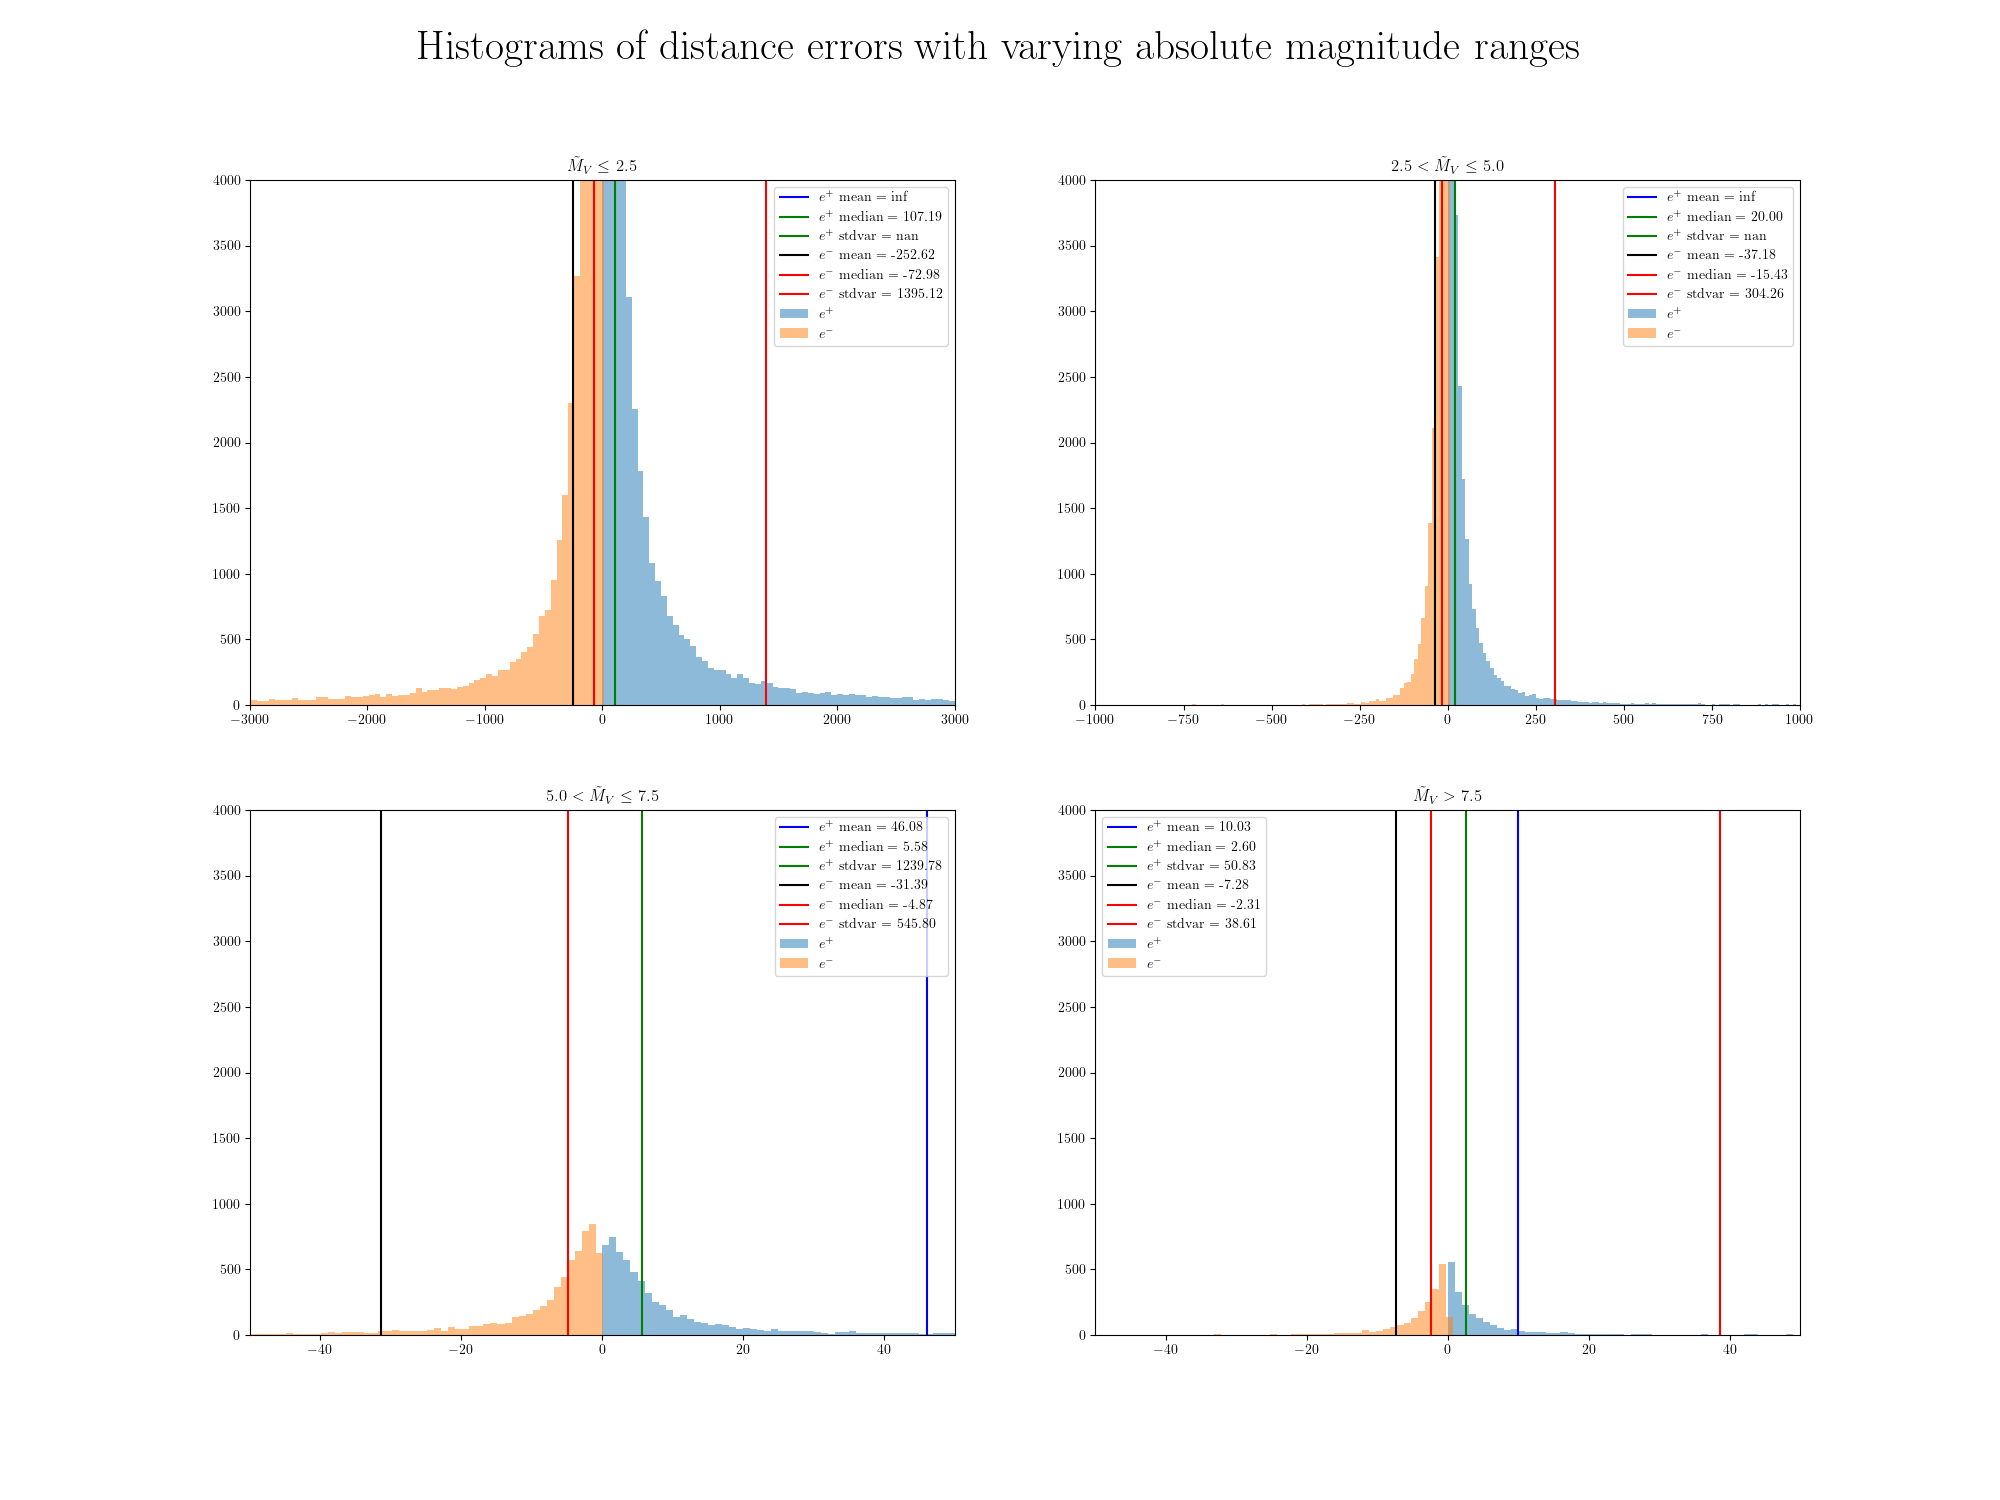
\includegraphics[scale=.33]{figures/e_Dist_hist.png}
			\caption{Distance Uncertainty Histogram (with magnitudinal ranging)}
		\end{figure}

		Of immediate interest - though perhaps expected - is that the mean uncertainty here is actually 0. In anycase, we get a good idea of the average errors present on either side of the curves (they are quite small, so we can be fairly confident in our prior results). 
		
\pagebreak		
		To get a better idea of the affect the uncertainty should have on our level of confidence in the above results, we can look at the ratio of the uncertainty of each distance measurement to the distance itself:
		
		\begin{figure}[h!]
			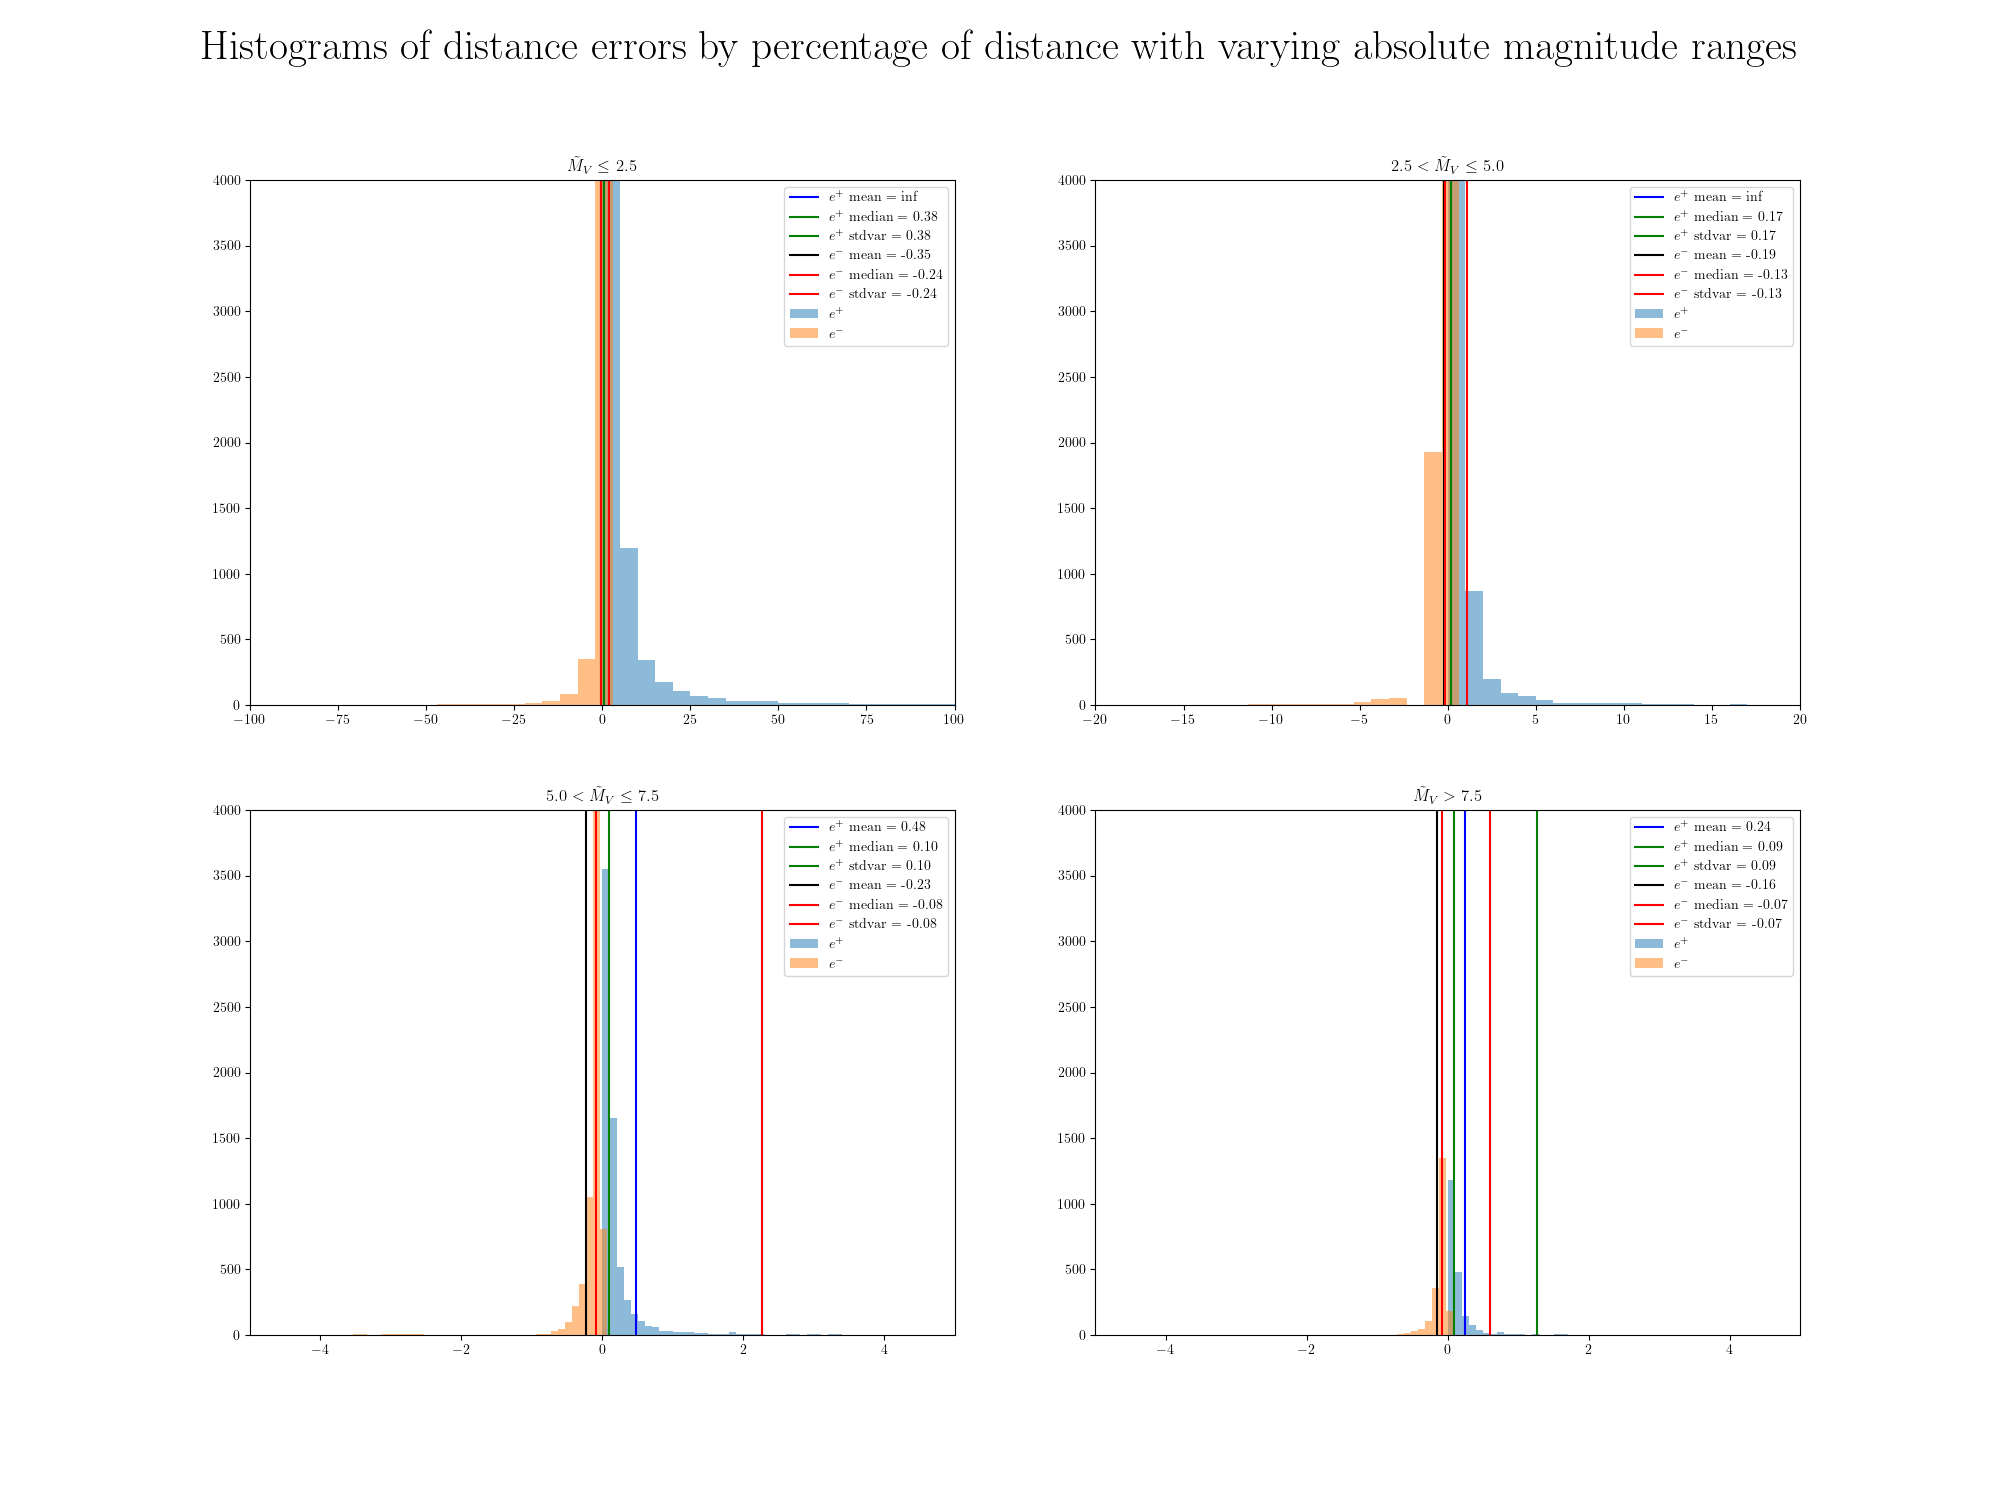
\includegraphics[scale=.33]{figures/e_Dist_perc_hist.png}
			\caption{Distance Uncertainty Histogram (by percentage of distance, with magnitudinal ranging)}
		\end{figure}
		
		This is an astounding result: it appears that the brightest stars - which one would imagine would be the easiest to measure given the all of the light that can be captured - actually has the most uncertainty in its measurements within the specified region, whereas the dimmer stars actually have fairly small percent uncertainties on their distance measurements.
%\pagebreak		
%		Here is a t-test performed on the distances of stars at $M_V \in (2.5,5.0]$
%		\begin{figure}[h!]
%			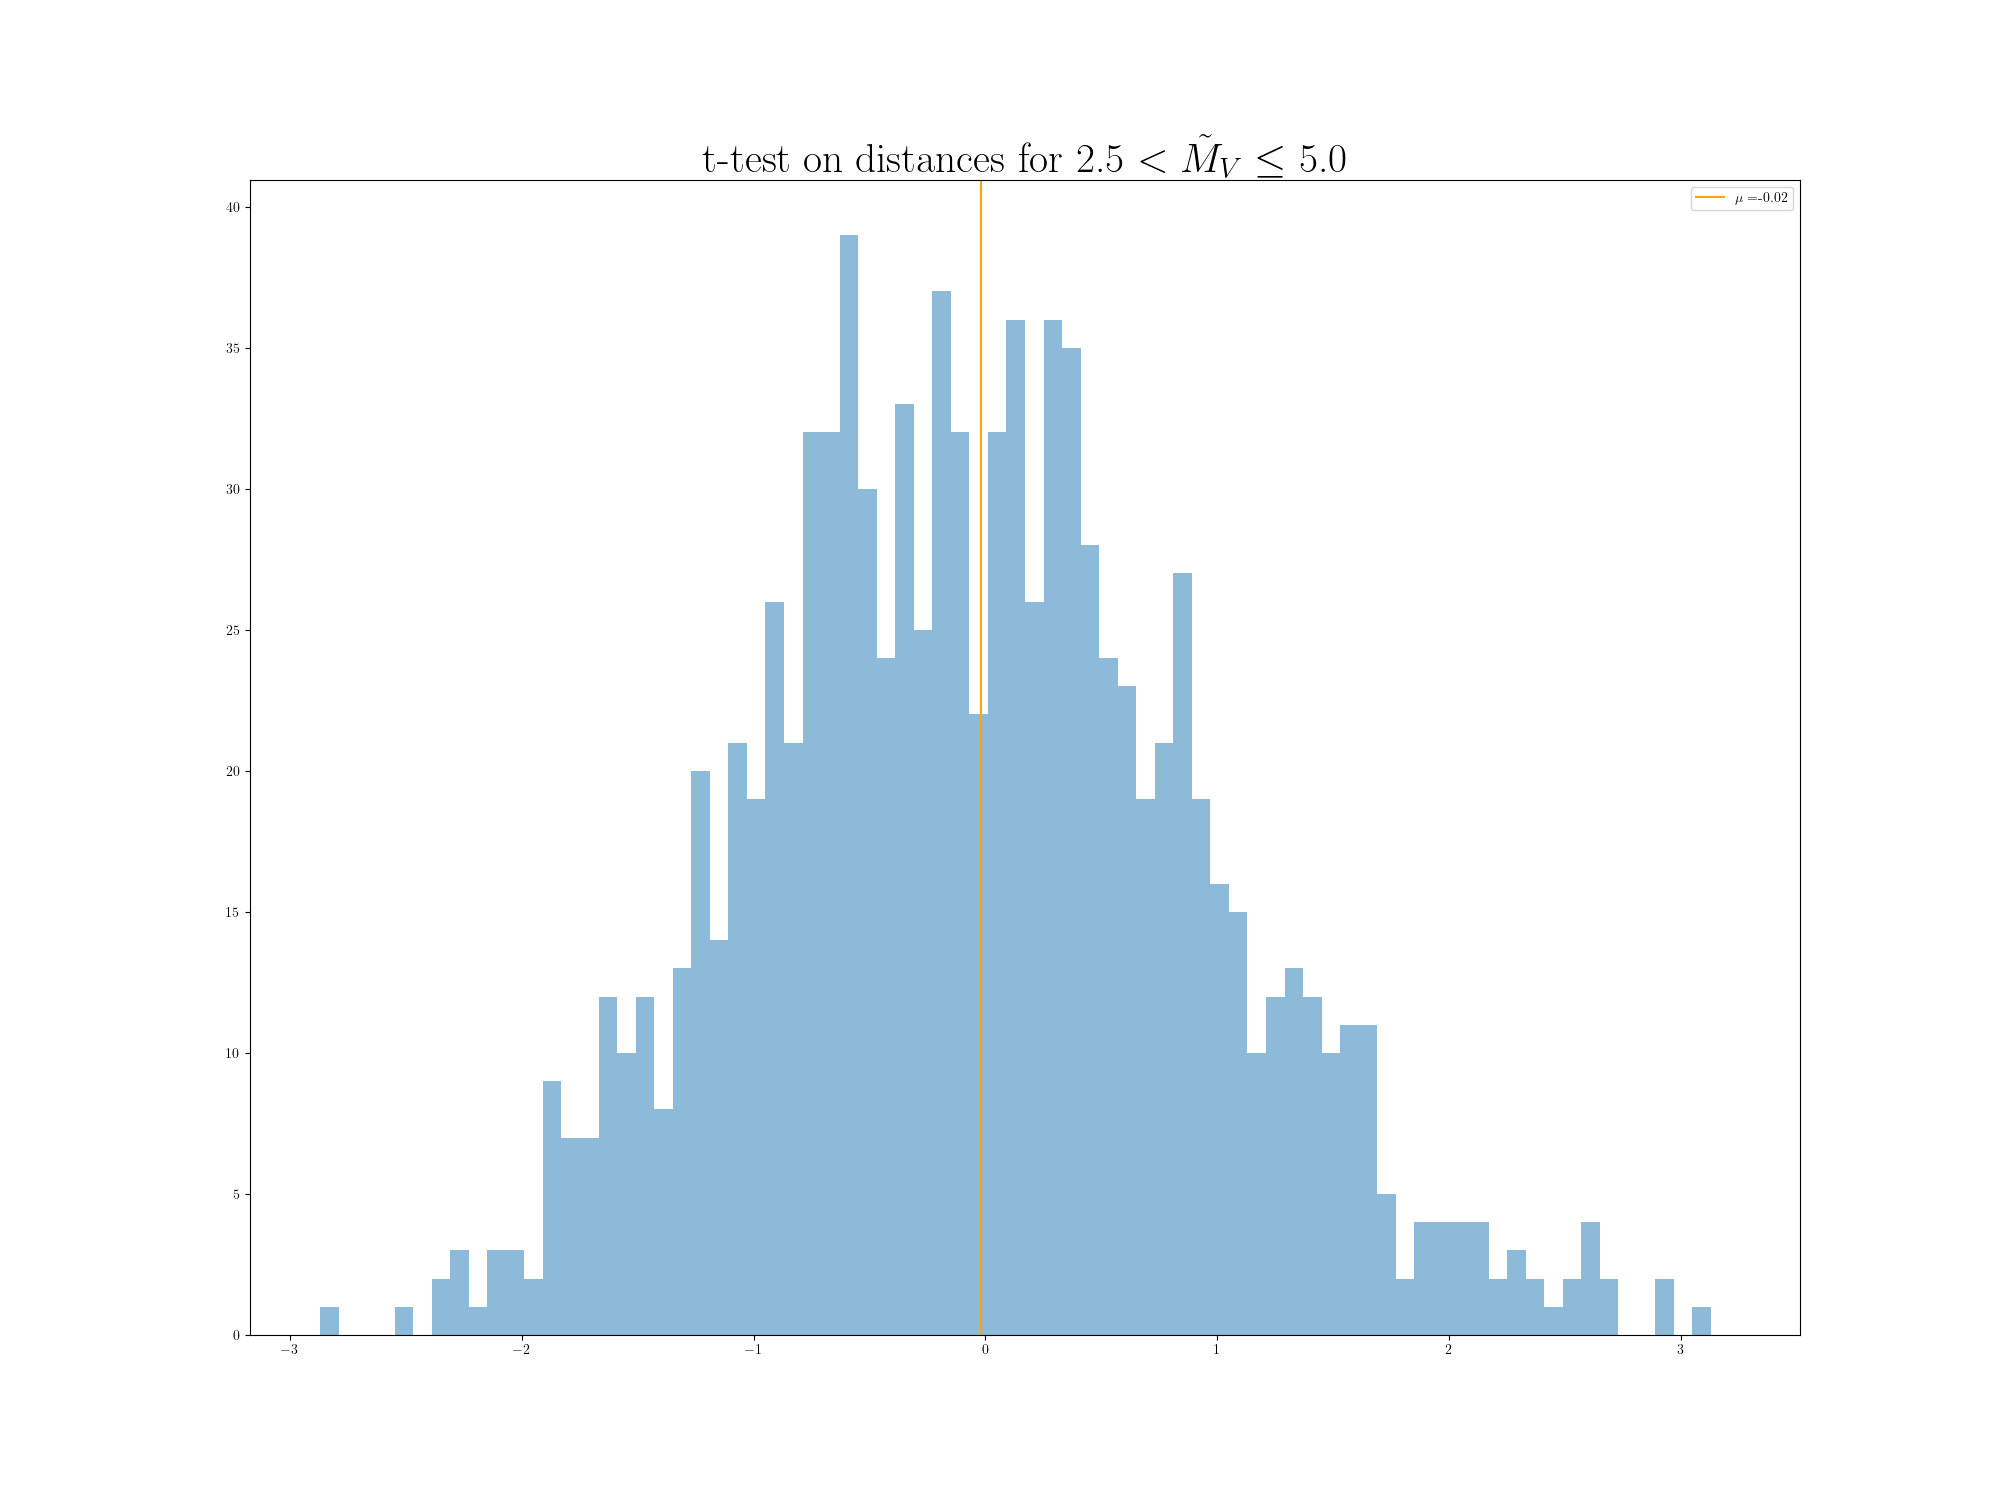
\includegraphics[scale=.33]{figures/ttest_hist.png}
%			\caption{}
%		\end{figure}
		
\pagebreak
		To get perhaps a broader view of the overall completeness of the hipparcos catalog, we can look at a plot of the distance vs. absolute magnitude plot:
		
		\begin{figure}[h!]
			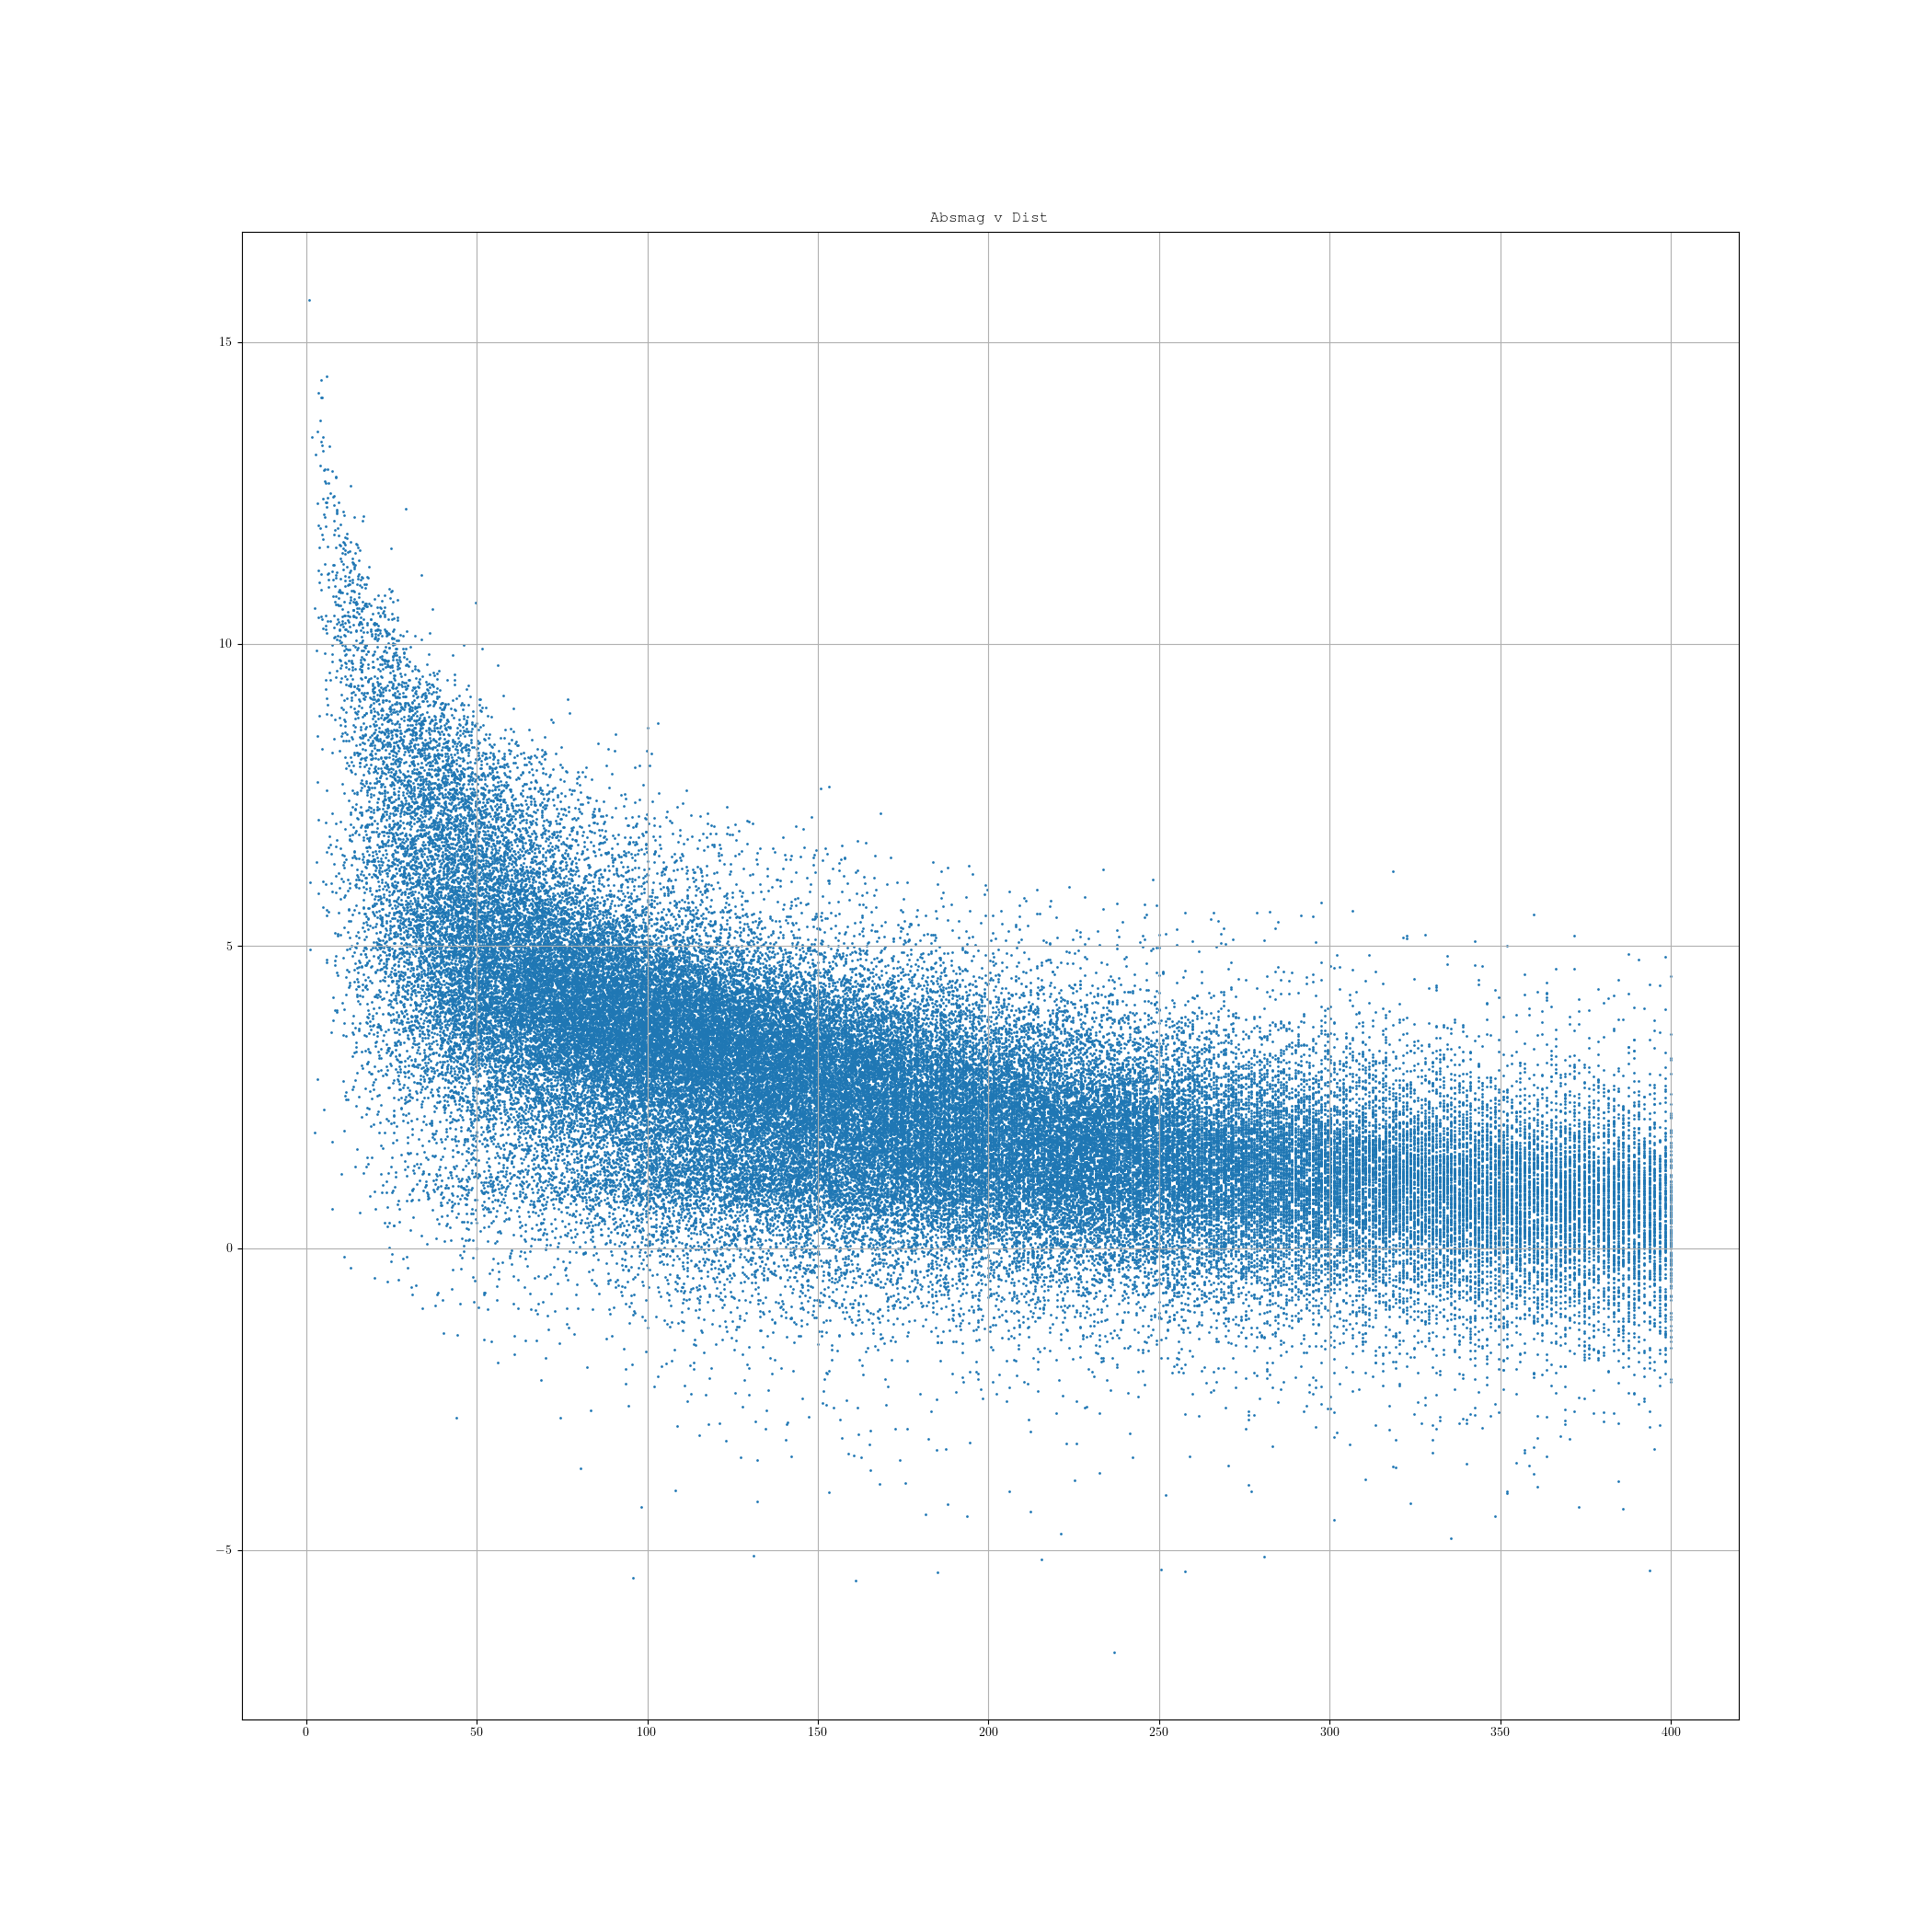
\includegraphics[scale=.33]{figures/dist_mag.png}
		\end{figure}
\pagebreak
		Which shows that the as we see farther away from Sol, dimmer stars become less and less visible. We don't expect dimmer stars to become less frequent as distance increases, so this reinforces the idea that the Hipparcos catalog is incomplete at 400 pc. This suggests that the catalog may not be complete even past 10 pc, but that for stars with $M_V\le 8$ it remains possible that it is complete out to 50 pc.
		
		Of interest to note: the cluster seems to have a centerline asymptote of $M_V=0$, which it approaches fairly rapidly. Given this, it would appear that there is some form of completeness in the catalog - though it is obvious that the overall density seems to drop, and the precision of the distance measurement seems to decrease as well (shown by the vertical grating that occurs around 300+ pc) 
		
		
\pagebreak
	\section{Conclusions}
		
		Overall, the results of this exercise seem to point to the \textit{possibility} that the Hipparcos catalog may be complete upto about 10 pc away from Sol in general, and within some magnitude bands could even be complete as far away as 300 pc (though this is for the brightest regime of stars, which as we found have the greatest uncertainties, thus lowering our overall confidence in this conclusion).
		
		We used this idea of a triangular distribution to build confidence in the possibility of completeness, and in general we found that the population of data could quite possibly be complete upto 50 pc, and when we broke the population into magnitude bands, this mark varied significantly to either side - with the possible completeness distance of 10 pc for the $M_V>7.5$ band having the highest confidence due to the mean uncertainty on the distance measurement being around .3\%, where as are lowest confidence mark would be the 300 pc distance for the $M_V\le 2.5$ band, since the uncertainty on its distance measurements had an rms of
		
		This preliminary analysis shed light on a few interesting characteristics of the Hipparcos catalog - and perhaps the function of astrometry in general - that we believe deserve deeper study, and so naturally the next step would be to dive further into an analysis of the uncertainty values in order to gain a deeper understanding of how that might effect our confidence and completion distances, which should end up giving us a better answer as to if and how complete the catalog is. 
		The immediate extension of this would be to first take a deeper look at the data to narrow down where the infinite values are coming from - since we use the $\tan$ function to calculate distance, the infinite values in the statistics here are likely coming from the fact that some of the uncertainties are very close to a vertical asymptote, and so the numpy trig library is unable to give us back a finite value. Furthermore, we need to perform a more in-depth look as to whether or not the uncertainties are consistent - this particular task could be entire project in and of itself. Finally, quantifying the completeness of the catalog more precisely - which in the case of this project was out of scope due to the complexity of the error analysis that needed to be performed in order to provide any decent level of confidence to whatever results we obtained. 
		In any case, we have laid an excellent groundwork from which to continue building a mechanism by which a quantitative analysis of a star catalog can be performed based on the data contained within the catalog itself - with as few external assumptions as possible.

%%%%%%%%%%%%%%%%%%%%%%%%%
\pagebreak
\nocite{vizier}
\nocite{nasa}
\nocite{cosmos}
\nocite{brit}
\bibliography{ref}
\bibliographystyle{plain}
\end{document}